\documentclass{article}

\usepackage[english]{babel}
\usepackage{microtype}
\usepackage{graphicx}
\usepackage{wrapfig}
\usepackage{enumitem}
\usepackage{fancyhdr}
\usepackage{amsmath}
\usepackage{chemformula}
\usepackage{index}
\usepackage{hyperref}
\usepackage[margin=1.0in]{geometry}
\usepackage{qtree}
\usepackage{float}
\usepackage{booktabs}
\usepackage{tabularx}
\usepackage{textcomp}
\usepackage{multicol}

\begin{document}
\title{Summary: Nervous System Structure and Function}
\author{Dowland Aiello}
\date{April 13, 2020}

\maketitle
\tableofcontents
\fancyhf{}

\newpage

\section{Overview: actors and structures of the nervous system}

\subsection{Structure of the Neuron}

In contrast with the chemical message-reliant \textbf{endocrine} system,
the \textbf{nervous system} is capable of quickly conveying particular
messages to and from different actors in the body through \textbf{neurons}---
chemically and electrically signaling nerve cells. Typically, a neuron consists
of:

\begin{itemize}
	\item A \textbf{cell body} containing the nucleus and organelles
	\item Extensions that convey signals
\end{itemize}

In some cases, a \textbf{neuron} may be referred to as a \textbf{nerve}, should
it be wrapped in connective tissue.

\subsection{Structure of the Nervous System}

\begin{wrapfigure}{l}{0.4\textwidth}
	\centering
	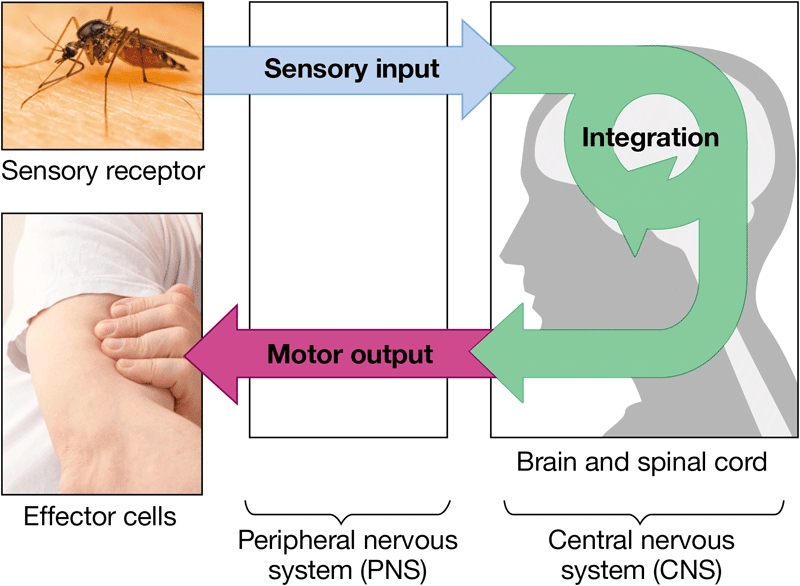
\includegraphics[width=1.0\linewidth]{goals_of_nervous_system.png}
	\caption{The three functions of the nervous system, exemplified in the human body.}
\end{wrapfigure}

The nervous system can be divided into two spatially distinct systems: the
\textbf{central nervous system (CNS)} and the \textbf{peripheral nervous
system (PNS)}. The former of the aforementioned anatomical divisions---the CNS
---is comprised by the \emph{brain} and the \emph{spinal cord} (where
applicable). The latter consists of neurons that work in conjunction with the
CNS to transmit and convey information through the body. These systems function
with the goal of providing utility with respect to three functions:

\begin{enumerate}
	\item \textbf{Sensory input}: the flow of signals from sensory receptors,
		through the PNS to the CNS
	\item \textbf{Integration}: the formation of appropriate responses to 
		certain stimuli
	\item \textbf{Motor output}: the application of responses generated through
		integration via \textbf{effector cells} (e.g., muscle, gland cells)
\end{enumerate}

In the nervous system, implementation of these three functions is achieved through
the utilization of three distinct classes of neruons: \textbf{sensory neurons},
\textbf{interneurons}, and \textbf{motor neurons}. Sensory neurons are
responsible for making data collected from the sensory receptors available to the
central nervous system. Of course, this data must \emph{integrated}. This is
achieved by the interneurons. The last of the aforementioned functions, motor output,
is provided by motor neurons, which apply responses generated through integration
via effector cells.

For example, consider the pathway of data from the outside world to effector cells
with respect to a \textbf{reflex}, such as the ``knee jerk:''

\begin{multicols}{2}
	\begin{enumerate}
		\item A tendon in the knee is tapped
		\item The quadricep muscles are stretched
		\item The stretch is detected by a sensor receptor
		\item The stretch is conveyed to the spinal cord via a sensory neuron
		\item A motor neuron in the CNS receives data regarding the ``tap''
		\item Several interneurons are made aware of the event
		\item A motor neuron signals the quadriceps to contract
	\end{enumerate}
\end{multicols}

\end{document}
